\chapter[Data and Methods]{Data and Methods}

This chapter starts with a small section on the research area \ref{area}.
Then, per research question a section is dedicated, describing its data, pre-preprocessing steps and the analysis. In section \ref{rq1} the methodology for literature studies and interviews is explained to find critical walkability factors (research question 1). Section \ref{rq2a} shows the data collection and pre-processing steps for the analysis of existing geo-data, research question 2. 
In section \ref{rq2b} the data collection and pre-processing steps for the collection of our own geo data, with GPS devices and an accelerometer are explained followed by the steps for analysing this data (research question 3). The changepoint methods for comparing the existing geo-data with the own collected data is explained in section \ref{rq2c}. Changes in the time series of the rollator walks are detected and plotted on the map to compare the data sources (research Question 4).

\clearpage
\section{Study area}\label{area}
This project in conducted for the project MeetRollator in the scope of the recently founded Amsterdam Institute For Advanced Metropolitan Solutions (AMS). The study area of AMS in Amsterdam, see left figure \ref{kaart} for the location. The Amsterdam Municipality contributed with data that covers the centre area of Amsterdam, indicated with the red square in the right figure \ref{kaart}. 
The literature study, interviews, AHN study will be mostly focussed on this area. The more general measurements were taken in Wageningen due to a more conventional location and travelling circumstances for the conducting researcher. See figure \ref{tracks} from chapter 3.5. 

\begin{figure}[h]
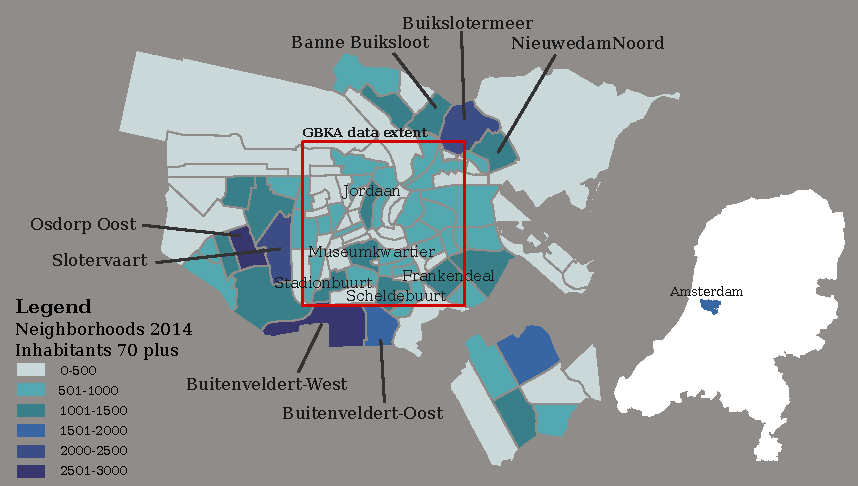
\includegraphics[width=\textwidth]{img/M1_StudyArea.pdf}
\centering
\caption{Study area Amsterdam, The Netherlands\label{kaart}}
\end{figure}

There is no exact information on the amount of elderly using a rollator in Amsterdam or where they live. There for the CBS statistics of 2013 were used to detect the neighbourhoods were the most elderly above 70 live. In figure \ref{kaart} can be seen that in the centre the most elderly live in the Jordaan. In the whole of Amsterdam the most elderly can be found in the South West and North. 